\subsection{Difusi�n}
\begin{frame}
\frametitle{}

\begin{figure}
\begin{tikzpicture}[node distance=0.5cm, auto,>=latex', thick]
\scriptsize
    % We need to set at bounding box first. Otherwise the diagram
    % will change position for each frame.
    \path[use as bounding box] (-1.5,0) rectangle (12,-2);

    % TT methodology     
    \node [phase]                        (monitoreo)     {Vigilancia};
    \node [phase, below of=monitoreo]    (choice)        {Elecci�n};
    \node [phase, below of=choice]       (acquisition)   {Adquisici�n};
    \node [phase, below of=acquisition]  (adaptation)    {Adaptaci�n};
    \node [phase, below of=adaptation]   (absortion)     {Absorci�n};
    \node [phase, below of=absortion]    (aplication)    {Aplicaci�n};
    \node [phase2,below of=aplication]   (difusion)      {Difusi�n};

    %%%%%%%%%%%%%%%%%%%%%%%%%%%%%%%%%%%%%%%%%%%%&
    %            Difusi�n
    %%%%%%%%%%%%%%%%%%%%%%%%%%%%%%%%%%%%%%%%%%%%&


    \onslide<1> \node [difusion_es, right=1cm of absortion.east] (est_difusion)      
      {
       \begin{center} \textbf{El conocimiento como bien p�blico} \end{center}
       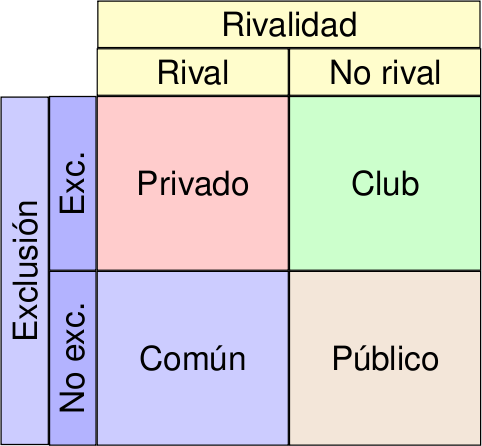
\includegraphics[scale=.4]{../images/bienes_clasific.png}\\
       
        \noindent{Ecuaci�n costo-beneficio de Ostrom:\hfill} \\
        \noindent{$ BC > BN + C $\hfill \\
        BC: Beneficio a contribuir.\hfill \\
        C : Costo de la contribuci�n.\hfill \\
        BN: Costo de no contribuir.\hfill}
      };

    \onslide<2> \node [difusion_es, right=1cm of absortion.east] (est_difusion)      
      {
       \begin{center} \textbf{Marco para analizar el conocimiento como bien p�blico aplicado a la metodolog�a propuesta} \end{center}
       \begin{center} 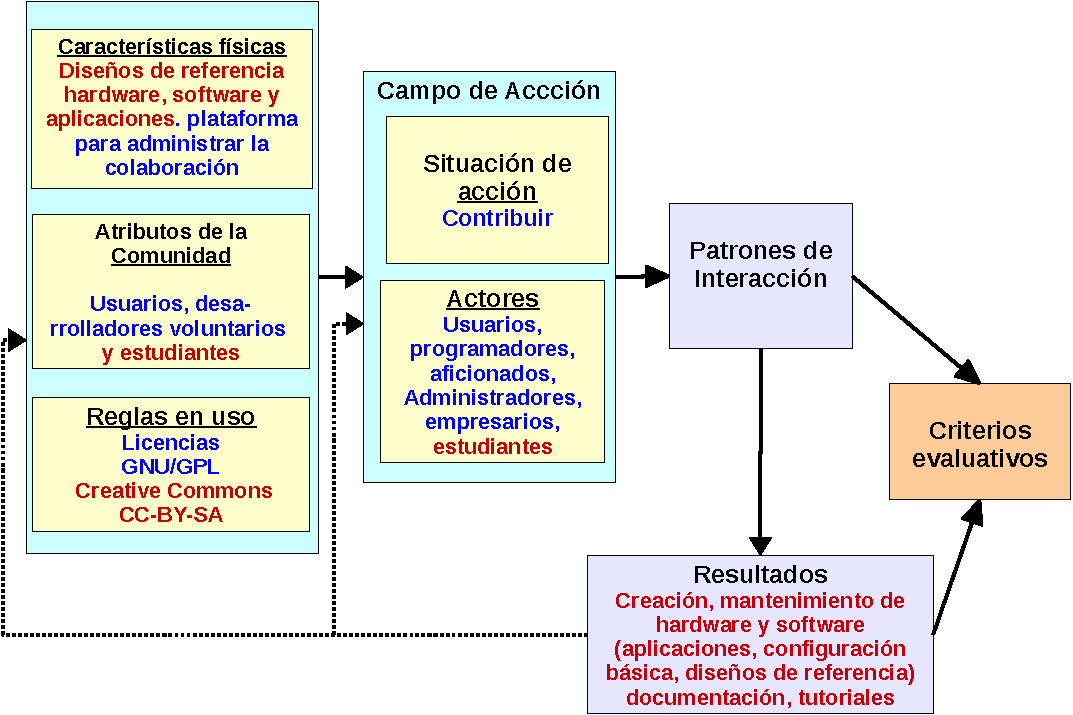
\includegraphics[scale=.39]{../images/framework_hwcl.pdf} \end{center}
      };

    \onslide<3> \node [difusion_es, right=1cm of absortion.east] (est_difusion)      
      {
       \begin{center} \textbf{Marco para analizar el conocimiento como bien p�blico aplicado a la metodolog�a propuesta} \end{center}
       \begin{center} 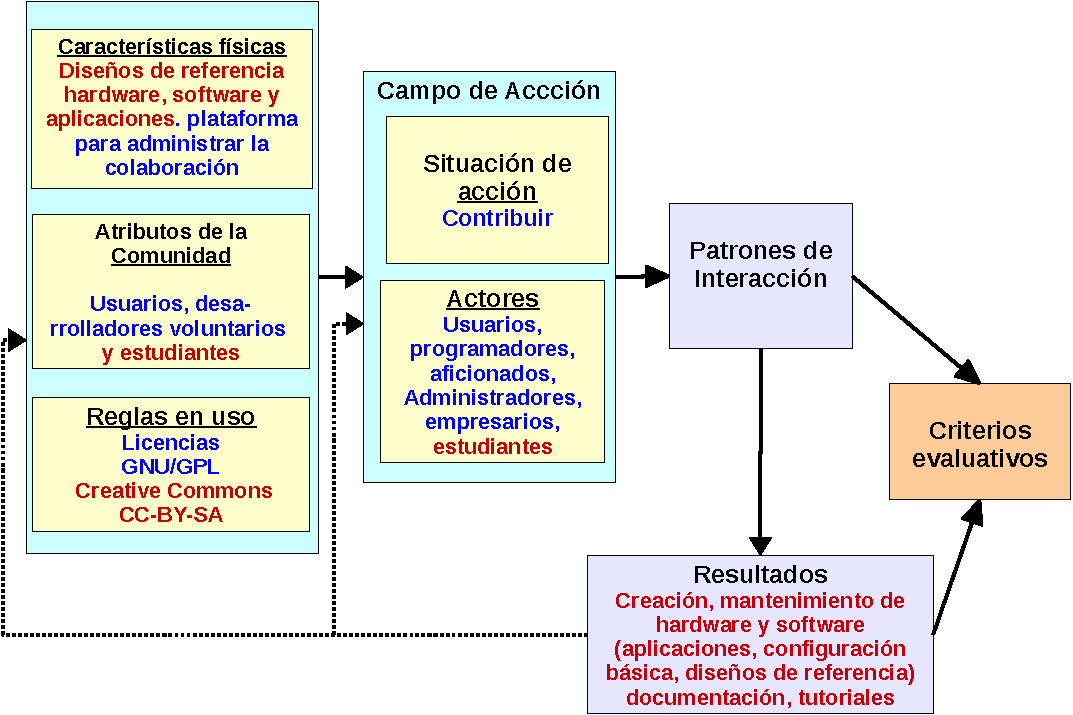
\includegraphics[scale=.39]{../images/framework_hwcl.pdf} \end{center}
      };



    %%%%%%%%%%%%%%%%%%%%%%%%%%%%%%%%%%%%%%%%%%%%&
    %        Estrategias de difusi�n
    %%%%%%%%%%%%%%%%%%%%%%%%%%%%%%%%%%%%%%%%%%%%&
    \onslide<4> \node [difusion_es, above right=2cm of adaptation.east] (est_difusion)      
      {
       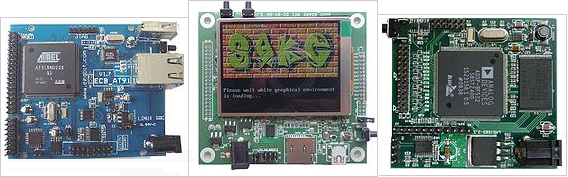
\includegraphics[scale=.25]{../images/plataformas_hwcl.png}\\
       \color{blue!40!black} {Repositorios + Tutoriales + Cursos en l�nea}
      };
    \onslide<4> \node [difusion_es, below = 0.5cm of est_difusion] (canales_difusion)      
      {
       \color{red!60!black} {Canales de difusi�n} \\
                          GIT, WIKI, MAIL\\
        \color{green!60!black}{C�digo fuente (.c,.v,.vhd,.S,.java), archivos de dise�o} 
      };
    \onslide<4> \draw[myarrow] (est_difusion.south) -- (canales_difusion.north);	
    
    \onslide<4> \node [phase2, below = .6cm of canales_difusion] (dif_academia2)      
      {
        Academia \\
        \begin{itemize}
         \scriptsize
         \item UIS, ULA, USTA, UDFJC, ENAP.
         \item ET-ITC.
         \item SEB.
        \end{itemize}
      };
    \onslide<4> \draw[myarrow] (canales_difusion.south) -- (dif_academia2.north);	

    \onslide<4> \node [phase2, left = .1cm of dif_academia2] (dif_academia)      
      {
        I+D UNAL \\
        \begin{itemize}
         \scriptsize
         \item Medicina
         \item Veterinaria
         \item Mecatr�nica
         \item Sistemas
        \end{itemize}
      };
    \onslide<4> \draw[myarrow] (canales_difusion.south) --++(0,-0.2)--++ (-2.3cm, 0) -- (dif_academia.north);	

    \onslide<4> \node [phase2, right = .1cm of dif_academia2] (dif_industria)      
      {
        Industria\\
         \scriptsize
        \begin{itemize}
         \item emQbit.
         \item $\mu$Ensamble.
        \end{itemize}
      };
    \onslide<4> \draw[myarrow] (canales_difusion.south) --++(0,-0.2)--++ (2.3cm, 0) -- (dif_industria.north);	
    
\end{tikzpicture}
\end{figure}

\end{frame}